\chapter{Experiments}

There are many possible designs for future lepton colliders \cite{Lipton:2012du,Koratzinos:2014cla} however here we focus on the two most developed projects, \ac{CLIC} and \ac{ILC}. Both projects are linear colliders which propose using electron-positron collisions and were founded over twenty years ago, though \ac{ILC} is currently the more mature design of the two. We will also discuss the detectors proposed for both experiments. \ac{ILC} currently has two detector concepts being developed, \ac{ILD} and \ac{SiD}, which will be operated in a 'push-pull' scheme in which both detectors are placed on a single platform that is periodically moved to alternate which detector is placed in the path of the beams. This is necessary as there is only one interaction point at a linear collider. Having two detectors has the advantage that any results made with one detector can be verified with the second to help reduce any systematic bias from either machine, however it comes with the penalty that each detector will only be able to take data half of the time and the process of moving the detectors in and out is lengthy ($\sim$ 3-4 days) resulting in reduced time for data taking for the experiment. \ac{CLIC} intends to operate with only one detector, a variation of the \ac{ILD} developed for \ac{ILC}, adapted for the different beam conditions present at CLIC. 

\section{ILC}

The ILC (\reffig{Fig:ILC}) is a proposed experiment consisting of a 31km ${e^+e^-}$ collider to be built in Kitakami in the northern region of Japan. The current construction schedule predicts the experiment will be finished in the mid 2020s with a cost of the order \pounds6 billion and will run for approximately 20 years. However, until funding is secured for the experiment this is just an estimate. The \ac{ILC} \ac{TDR} \cite{ILCTDR} was released in 2013 and gives a full description of the experiments' baseline design. While the \ac{TDR} is highly detailed, because the experiment is still under development it is possible that some of the information contained within it will become outdated and change before construction takes place. For simplicity any figures given in this section can be assumed to be taken from the \ac{TDR} unless otherwise stated.

\begin{figure}
  \centering
  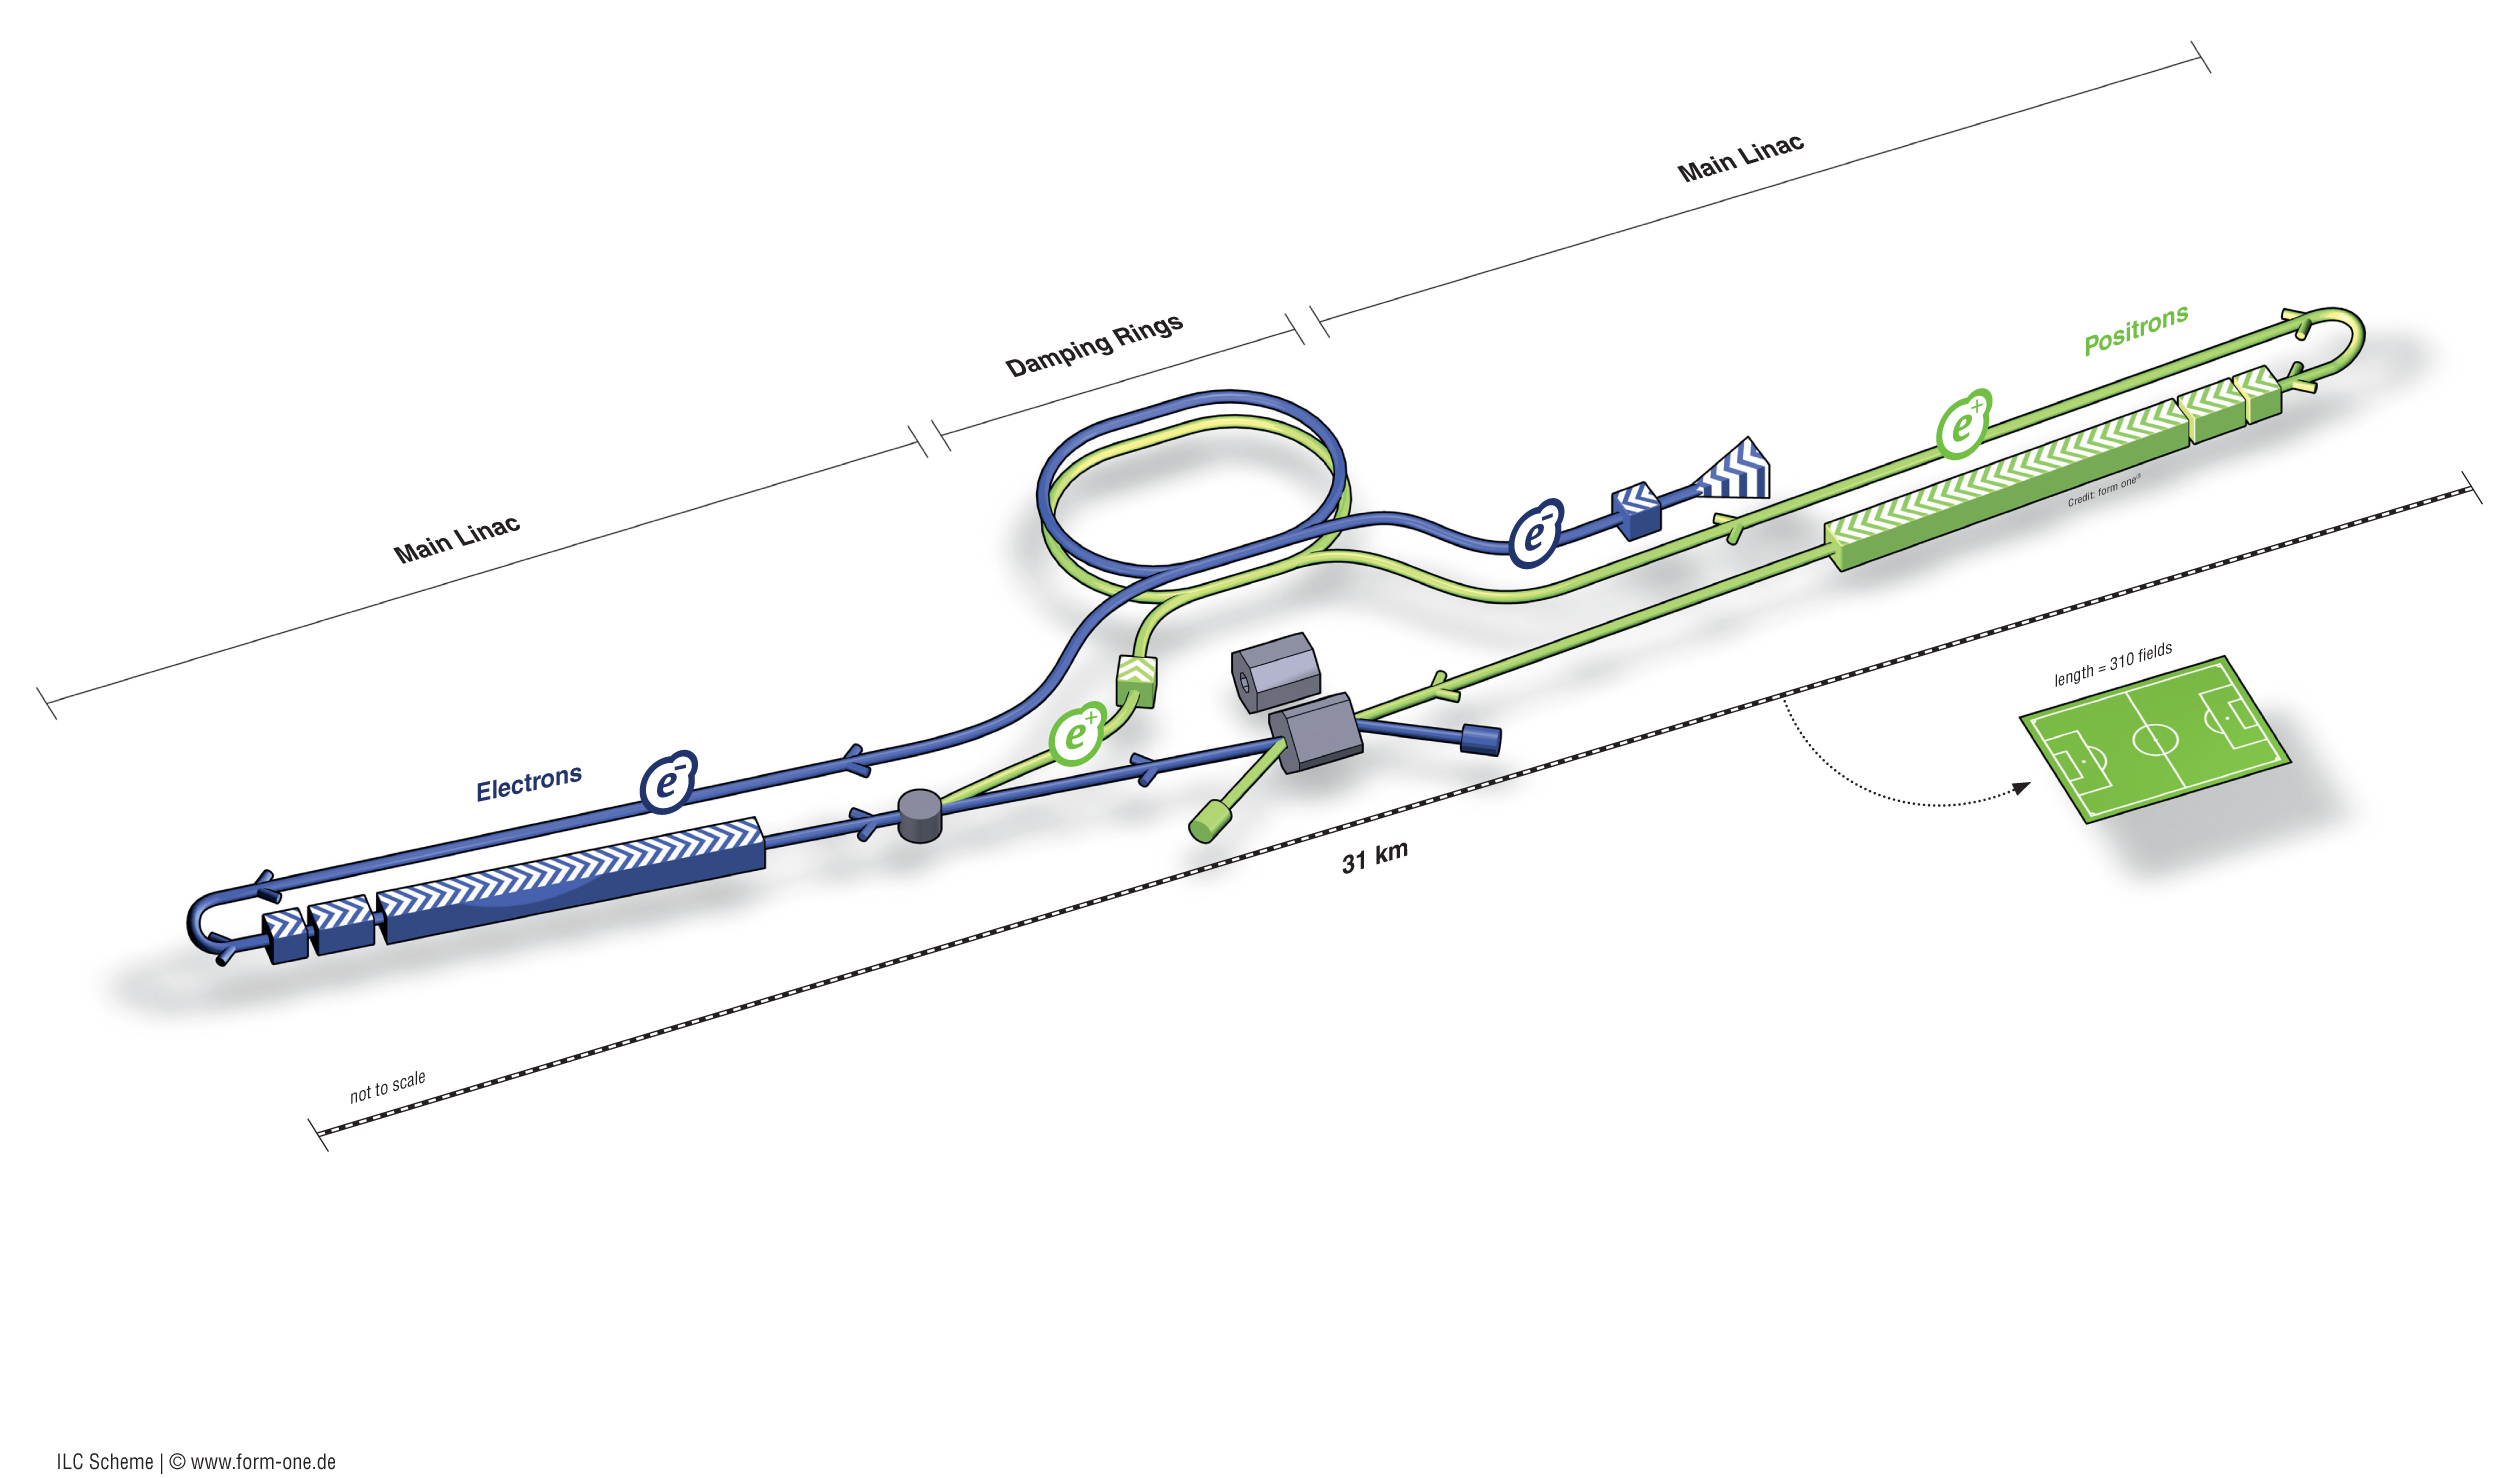
\includegraphics[width=0.9\textwidth,keepaspectratio]{Experiments/fig/ILC}
  \caption[The ILC Experiment]{The \ac{ILC} Collider\cite{ILCTDR}}
  \label{Fig:ILC}
\end{figure}

\subsection{Energy Staging}

The \ac{ILC} will first be built with a maximum collision energy capability of 500 GeV but with the potential for a later upgrade to 1 TeV which would require doubling the length of the machine to 62 km. The decision of whether the 1 TeV upgrade is necessary will largely be determined by the results of the \ac{LHC} experiments; if any new physics is discovered above 500 GeV then the 1 TeV upgrade could be essential to characterise it. Assuming the 1 TeV upgrade is realised the energy staging will be as described below.

The first three years will involve the ILC running at an energy of 250 GeV and taking 250 fb${^{-1}}$ of data. The main aim at this stage will be to measure the Higgs mass and ZH cross section from the Higgsstrahlung process as described in Chapter \ref{theory} to allow model independent measurements of the Higgs couplings to be performed.

For the following three years, the collider will then run at 500 GeV and will accrue a further 500 fb${^{-1}}$ of data. The main aims here will be to measure the HWW coupling, the total Higgs width and the absolute Higgs couplings to fermions. At this energy, measurements of top physics will also be possible including the top forward backward asymmetry. Outside of the Higgs sector, the top quark is perhaps the least well measured of the standard model particles and so provides another area in which to look for deviations from the standard model predictions.

After this there will be an upgrade to 1 TeV followed by another three years of data taking accumulating 1000 fb${^{-1}}$ of data. The aim of running at this high energy will be to search for new particles such as dark matter candidates and supersymmetric particles while improving upn the precision of the measurements performed at the lower energies. If one of these (or something entirely new) has already been discovered at the \ac{LHC} then the choice of 1 TeV might be scaled to match the scale of the newly discovered physics.

After this the collider will undergo a high luminosity upgrade and will run at the same energies for the same time periods for another 9 years but instead accruing 900, 1100 and 1500 ${fb^{-1}}$ at the respective energies. This will allow for a further increase in the precision of all measurements taken during the lower luminosity run.
While the \ac{TDR} proposes the above run scheme for the \ac{ILC} there is still debate about what energies should be used with arguments being made for running at 90 GeV (the Z mass) to gain precision measurements of the Z boson, 350 GeV (the top production threshold) to better measure the properties of the top quark or to simply only run at 250 GeV to provide precision Higgs measurements for minimal cost.

\subsection{Beam Production, Acceleration and Focusing}
\label{ILC:BEAM}

\begin{figure}
  \centering
  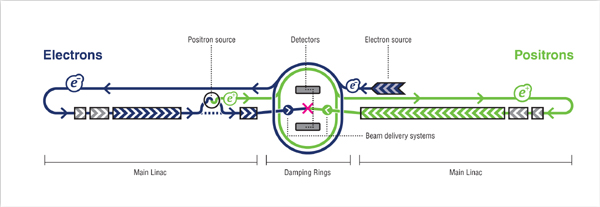
\includegraphics[width=0.9\textwidth,keepaspectratio]{Experiments/fig/ILC_Simplified}
  \caption[Schematic of the ILC accelerator layout]{A simplified schematic of the ILC\cite{ILCTDR}}
  \label{Fig:ILCsimple}
\end{figure}

\begin{table}
\caption[ILC Beam Parameters]{ILC Beam Parameters}
\label{table:ilcbeamparameters}
\centering
\begin{tabular}{l l l l l }
\toprule
\textbf{Parameter}                  & \textbf{Symbol}         & \textbf{Unit}& \textbf{Stage 1} & \textbf{Stage 2} \\
\midrule
Centre-of-mass energy               & $\sqrt{s}$                &GeV                                        & 250 & 500 \\
Repetition frequency                & $f_{\text{rep}}$        &Hz                                         & 5 & 5 \\
Number of bunches per train         & $n_{b}$                 &                                           & 1312 & 1312 \\
Number of particles per bunch                    & $N$                     &$10^{10}$                      & 2.0 & 2.0 \\
Bunch separation                    & $\Delta t_b$             &ns                                         & 554 & 554 \\
\midrule
Accelerating gradient               & $G$                     &MV/m                                       & 14.7 & 31.5 \\
Electron Polarization               & $P_-$                   &\%                                       & 80 & 80 \\
Positron Polarization               & $P_+$                   &\%                                       & 30 & 30 \\
\midrule
Total luminosity                    & $\mathcal{L}$           &$10^{34}\;\text{cm}^{-2}\text{s}^{-1}$     & 0.75 & 1.8 \\
Luminosity above 99\% of $\sqrt{s}$   & $\mathcal{L}_{0.01}/\mathcal{L}$    &                            & 87.1\% & 58.3\% \\
\midrule
IP RMS beam size                    & $\sigma_x/\sigma_y$     &nm                                         & 729.0/7.7 & 474/5.9 \\
RMS Bunch length                    & $\sigma_z$              &mm                                  & 0.3 & 0.3 \\
Horizontal emittance                & $\epsilon_x$            &$\mu$m                                     & 10  & 10 \\
Vertical emittance                  & $\epsilon_y$            &nm                                         & 35 & 35 \\
Estimated power consumption         & $P_{AC}$                &MW                                & 122    & 163   \\
\bottomrule
\end{tabular}
\end{table}

A simplified schematic of the \ac{ILC} accelerating structure is shown above in \reffig{Fig:ILCsimple} while a summary of the key beam parameters is shown in \reftab{table:ilcbeamparameters}. The first stage of the acceleration process is the production of electrons. This is done using the photoelectric effect by firing photons onto a GaAs target to produce photoelectrons. These electrons then enter a 3.2 km long damping ring which accelerates the beam up to 15 GeV. The primary purpose of the damping ring is to produce a homogeneous beam of electrons with uniform energy and momentum. After the damping ring the electrons enter into a two stage bunch compressor which separates the electron beam into ${\sim}$1300 bunches, each containing ${2\times10^{10}}$ electrons, with each bunch being separated by 554 ns and a maximum beam pulse length of $\sim$ 1.6 ms. The overall intended collision rate of these pulses is 5 Hz, which means that the duration for collisions is less than 1\% of the collision rate. This has important consequences for the detector design as it means the detectors have a large period of time in which to relax after events. As the detectors do not need to be operating for 99\% of the time, it is considerably easier to cool them meaning the material budget for the cooling systems within them can be greatly reduced. Following the bunch compression the electrons enter the main 11 km linac where they are accelerated up to the nominal beam energy using 7,400 1.3 GHz superconducting niobium \ac{RF} cavities (see \reffig{Fig:cavity}). 

\begin{figure}
  \centering
  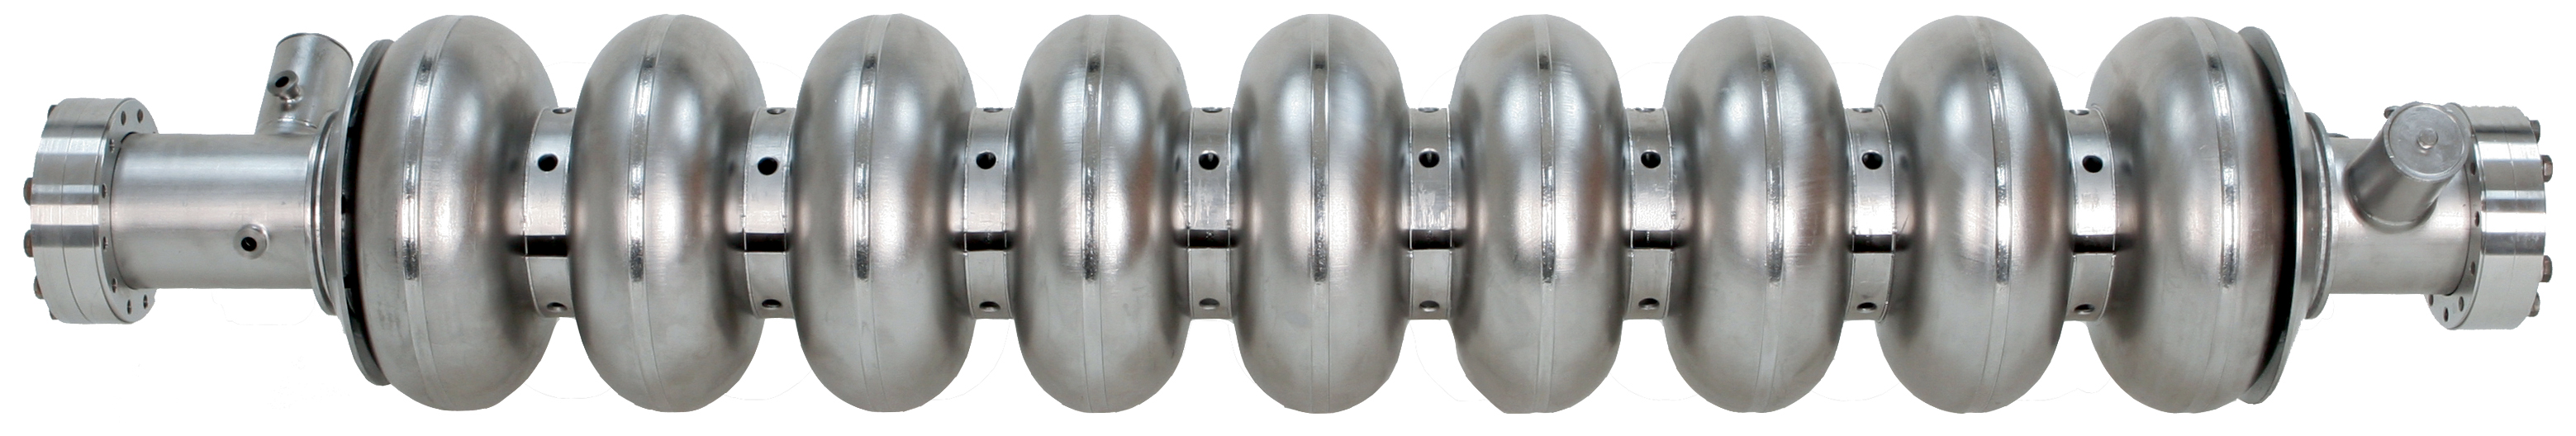
\includegraphics[width=0.75\textwidth,height=10cm,keepaspectratio]{Experiments/fig/Cavity}
  \caption[Superconducting Cavities For The ILC]{A 1.3GHz Superconducting Niobium Radio Frequency Cavity \cite{ILCTDR}}
  \label{Fig:cavity}
\end{figure}

The \ac{RF} cavities are kept at a temperature of 2K and act to produce an average accelerating gradient of up to 31.5MV/m (14.7MV/m for the 250GeV stage.)  The final stage before the collision is the \ac{BDS} which primarily acts to compress the beam into a ribbon shape with a cross-section of 7.7 x 729.0 nm while also handling the beam monitoring. The ribbon shape is designed to reduce \ac{BS} radiation from beam interactions while giving a small enough cross section that a high instantaneous luminosity can be achieved. Following the \ac{BDS} the beam finally enters the detector and collides with the oppposing positron beam at a crossing angle of 14 mrad then exits into the beam dump system which quenches what is left of the beam.

\subsection{Positron Production}
Positrons are produced at the \ac{ILC} by tapping off energy from the electron beam after it has been accelerated by the main linac. The electron beam is passed through an undulator which causes the electrons to emit synchrotron radiation in the form of 10-30 MeV photons by forcing the beam to take a rapidly varying path in the plane transverse to it's direction of motion. The resulting photons are then separated from the electron beam and are collided with a Titanium alloy target to produce electron positron pairs. The electrons and positrons are then separated and the electrons are dumped while the positrons are then passed into a damping ring and undergo all the same stages of acceleration and shaping as described above for the electrons.

\section{CLIC}

\begin{figure}
  \centering
  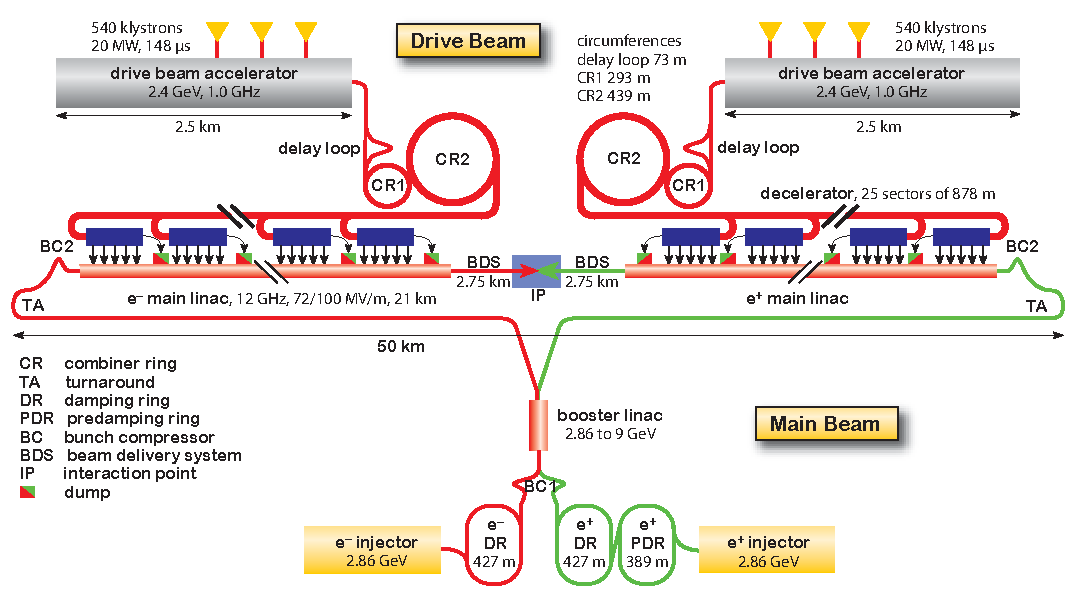
\includegraphics[width=0.75\textwidth,height=10cm,keepaspectratio]{Experiments/fig/CLIC-layout-3TeV}
  \caption[The CLIC Experiment]{The CLIC Collider. Layout for the CLIC accelerator at 3 TeV. For the lowest energy stage there will only be one drive beam constructed which will power both main beams\cite{CDR}}
  \label{Fig:CLIC}
\end{figure}

\begin{table}
\caption[CLIC beam parameters]{Parameters for the CLIC energy stages. The power consumptions for the 1.5 and 3\,TeV stages are from the CDR; depending on the details of the upgrade they can change at the percent level \cite{CLIC:2016zwp}.}
\label{table:clicbeamparameters}
\centering
\begin{tabular}{l l l l l l}
\toprule
\textbf{Parameter}                  & \textbf{Symbol}         & \textbf{Unit}& \textbf{Stage 1} & \textbf{Stage 2} & \textbf{Stage 3} \\
\midrule
Centre-of-mass energy               & $\sqrt{s}$                &GeV                                        & 380 & 1500 & 3000\\
Repetition frequency                & $f_{\text{rep}}$        &Hz                                         & 50 & 50 & 50\\
Number of bunches per train         & $n_{b}$                 &                                           & 352 & 312 & 312\\
Bunch separation                    & $\Delta\,t$             &ns                                         & 0.5 & 0.5 & 0.5\\
Pulse length                        & $\tau_{\text{RF}}$      &ns                                         &244 &244 &244\\
\midrule
Accelerating gradient               & $G$                     &MV/m                                       & 72 & 72/100 & 72/100\\
\midrule
Total luminosity                    & $\mathcal{L}$           &$10^{34}\;\text{cm}^{-2}\text{s}^{-1}$     & 1.5 & 3.7 & 5.9 \\
Luminosity above 99\% of $\sqrt{s}$   & $\mathcal{L}_{0.01}$    &$10^{34}\;\text{cm}^{-2}\text{s}^{-1}$     & 0.9 & 1.4 & 2\\
\midrule
Main tunnel length                  &                         &km                                         & 11.4 & 29.0 & 50.1\\
Number of particles per bunch                    & $N$                     &$10^9$                                     & 5.2 & 3.7 & 3.7\\
Bunch length                        & $\sigma_z$              &$\mu m$                                  & 70 & 44 & 44\\
IP beam size                        & $\sigma_x/\sigma_y$     &nm                                         & 149/2.9 & $\sim$ 60/1.5 & $\sim$ 40/1\\
Normalised emittance (end of linac) & $\epsilon_x/\epsilon_y$ &nm                                         & 920/20 & 660/20 & 660/20\\
Normalised emittance (at IP)        & $\epsilon_x/\epsilon_y$ &nm                                         & 950/30 & ---    &---\\
Estimated power consumption                        & $P_{\text{wall}}$         &MW                                & 252    & 364    & 589\\
\bottomrule
\end{tabular}
\end{table}

\ac{CLIC} is an experiment based at CERN which proposes the building of a 42 km accelerator at the main CERN site in Geneva (\reffig{Fig:CLIC}.) Despite being named as “compact”, \ac{CLIC} is actually longer than the initial 500 GeV \ac{ILC}. The reason for this naming is that \ac{CLIC} has a much higher accelerating gradient (100 MeV/m) compared to ILC and so provides a much higher energy per length. The expected build date for \ac{CLIC} is still relatively uncertain though is likely to be no earlier than 2030 as the accelerating technology required for \ac{CLIC} is less developed than that used by \ac{ILC}. This difference in the maturity of the two experiments can be seen from the fact that the \ac{ILC} has released its \ac{TDR} while the most comprehensive document for the CLIC project is still its \ac{CDR} \cite{CDR}. Updates on this document have been provided in the New Baseline Report \cite{CLIC:2016zwp} released in 2016 and any details specified here can be assumed to come from these two documents. 

Overall the design for \ac{CLIC} is relatively similar in layout to the \ac{ILC} but with a few changes. Positron production at \ac{CLIC} is done completely independently from the main electron beam, though they are still produced via the same mechanism as before. The \ac{BDS} still compresses the beam into a ribbon shape to give it a small cross-section and reduced \ac{BS}, however the aspect ratio is reduced compared to at \ac{ILC}. This results in larger contributions from beam photon radiations at \ac{CLIC}. The collision rate at \ac{CLIC} is significantly higher as it aims to be a high luminosity device- the collision rate will be 50 Hz with 354 bunches per pulse with a separation of just 0.5 ns. This means that CLIC will have a significantly higher duty cycle which will make cooling of the detectors harder and will give the detectors less time to relax after events. A summary of the beam parameters for CLIC is shown in \reftab{table:clicbeamparameters}. While these difference are important, the most significant changes are in the energy staging and acceleration technology used at \ac{CLIC} (see \refsec{sect:clicaccelerator}.)

\subsection{Energy Staging}

CLIC will operate at three energy stages- 380 GeV, 1.5 TeV and 3 TeV collecting 500 ${fb^{-1}}$, 1.5 ${ab^{-1}}$ and 2 ${ab^{-1}}$ of data respectively. During the running of the 380~GeV energy stage, construction of the 1.5~TeV structure will be carried out (and so on for the 1.5 TeV and 3 TeV scales) so as to reduce the delay between operation at successive energy stages. 

The 380 GeV energy scale is chosen as it is above the \ttbar production threshold and provides a significant cross section for many channels involving the top quark. This stage is also supplemented by a series of 10 measurements around the \ttbar threshold taking 10 ${fb^{-1}}$ each with the aim of measuring the top mass and width from the line shape of the \ttbar production cross section at threshold. The 380~GeV stage will also be used to provide measurements of the higgs boson similar to those performed at \ac{ILC} during it's two lower energy stages.

The 1.5 TeV energy stage provides the ability to further study the top and higgs in more detail with several new channels becoming significant e.g top yukawaw coupling, higgs self coupling, while the 3~TeV stage pushes the energy frontier allowing the possibility of direct detection of new physics at the multi-TeV scale. The choice of 3~TeV is based upon certain models of supersymmetry which predict new particles to exist at this energy (see \reffig{Fig:SuperSym}).

For clarification it should be stated that for many years the proposed scheme for CLIC was actually to operate at 500~GeV, 1.4~TeV and 3~TeV. These were updated to provide better precision on measurements of the top quark during the lowest energy stage (\ttbar production threshold is $\sim$ 350 GeV) and improved precision on the Higgs self-coupling during the second stage. It is important to be aware of these changes as the studies presented in chapters \ref{Higgs Analysis} and \ref{chapter:topanalysis} were both carried out at 1.4 TeV assuming the original energy staging, however it is expected that there will be negligible impact on the findings of these studies from changing the energy to 1.5 TeV.  

\begin{figure}
  \centering
  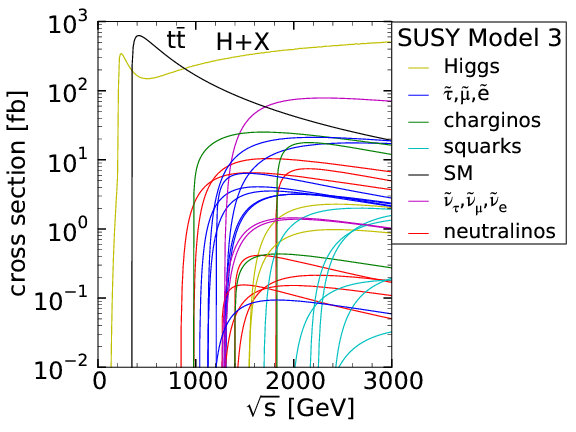
\includegraphics[width=0.75\textwidth,height=10cm,keepaspectratio]{Experiments/fig/clicSS}
  \caption[Cross Sections For Supersymmetric Processes at \ac{CLIC}]{Cross sections for production of various supersymmetric particles at an ${e^+e^-}$ collider as a function of centre of mass energy.}
  \label{Fig:SuperSym}
\end{figure}

\subsection{Acceleration Technology}
\label{sect:clicaccelerator}
Unlike \ac{ILC}, the acceleration technology will not be superconducting but will instead use two beams of electrons-- referred to as the main beam and the drive beam-- rather than just one main accelerated beam. The drive beam is accelerated using standard accelerating technology (klystrons) as in \ac{ILC} to accelerate bunches of electrons to 2.75 GeV. These bunches then enter a series of delay/control rings which are designed such that the electrons within them get combined with the new electrons being added from the drive beam accelerator to build up a large number of low energy electrons which combined carry a large amount of energy. The energy from this beam is then used to drive the main beam. This is done by rapidly decelerating the drive beam electrons down to 10\% of their initial energy and using the resulting \ac{RF} produced to accelerate the smaller number of electrons in the main beam resulting in a rapid acceleration. The main beam is then used to supply collisions. Overall the result is that the machine is simply acting as a novel form of transformer, converting a high current, low energy beam of electrons into a lower current, high energy beam. This approach allows for very high accelerating gradients but has the disadvantage that in approximately 1\% of events the sudden input of energy from the drive beam can cause electrical breakdowns in the main beam cavity, which disrupt the alignment and structure of the main beam making them unsuitable for use.

\section{Linear Collider Analysis Framework}

A common framework known as ILCSoft used for event simulation, reconstruction and analysis has been developed for both \ac{ILC} and \ac{CLIC} to allow for sharing of techniques between the two experiments. Here we will provide an overview of the key packages used.

\subsection{Event Generation}

Event generation is performed using an external package called WHIZARD \cite{Kilian:2007gr}. WHIZARD itself handles most of the event generation such as the calculation of hard matrix elements, phase space considerations and accounting for interference between processes, however for certain aspects it relies on additional packages. The most relevant of these are tau decays which are handed by TAUOLA\cite{Jadach:1990mz} and hadronization which is handled by PYTHIA\cite{Sjostrand:2006za}. Unfortunately no other hadronization package is available within WHIZARD which makes it challenging for evaluating systematic uncertainties arrising from how jets are modelled. The output from WHIZARD is a series of four momenta for all the particles produced in the collisions. These are then passed to a package called MOKKA whcih acts as an interface to GEANT4\cite{MoradeFreitas:2002kj}. Within MOKKA the interaction of the particles with the detector is modelled and a series of energy deposits are recorded for the various subdetector components. These are then finally passed on to the ILCSoft reconstruction package MARLIN in which digitisation of the hits and track reconstruction occur to produce realistic outputs from the detector. At this stage $\gamma\gamma\rightarrow$ hadron beam backgrounds are overlayed on the events assuming a rate of 1.6 events per bunch crossing.


\subsection{Pandora Particle Flow Algorithm}
\label{Pandora}

Pandora\cite{Thomson200925} is an advanced Particle Flow Algorithm used at linear colliders which allows an increased level of precision from detector measurements. The underlying principle behind particle flow is to try and always use the most precise detector component for performing energy measurements where possible. Typical values for energy resolutions for a charged particle in the main detector components are 10$^{-4} \times$ $E^2$ in the tracker, 0.15 $\times \sqrt{E}$ in the \ac{ECAL} and 0.55 $\times \sqrt{E}$ in the \ac{HCAL}. For a typical jet the composition will usually be $\sim$60\% charged hadrons, 30\% photons and 10\% hadrons. Traditionally for measuring the energy in a jet one would simply sum the deposits in both calorimeters resulting in a relatively poor energy resolution of $\sim$60\%/$\sqrt{E}$ due to the large component being measured in the \ac{HCAL}. If one can measure the charge hadron component in the tracker instead, this performance can be vastly improved to $\sim$20\%/$\sqrt{E}$. In order to be able to reach this performance, accurate association of tracks with deposits in the calorimeters is crucial. This is achieved by having a high granularity calorimeter and a high spatial resolution for the tracker. In practice however, even with a well designed detector, the particle flow algorithm can still fail to reconstruct the correct energy due to ambiguities referred to as ``confusion''. For example, if a photon enters the calorimeter near to a charged hadron, it is possible that the two will not be resolved and the energy identified from just using the track will neglect the contribution from the photon. Energy can also be overestimated in cases where a charged hadron showers in such a way that it looks like two separate calorimeter deposits which results in part of the shower being identified as a neutral hadron and the other fragment being associated with the track. One of the main design aims of the detectors will be to try and minimise these confusion effects. 


\section{Detectors}
The \ac{ILC} has been designed with the intention of having two unique detectors so that results can be validated by cross-checking between the two detectors. However, because \ac{ILC} is a linear collider it is only feasible to have one interaction point and as a result the beam time will have to be shared between the detectors. This will be done using a 'push-pull' design in which both detectors are placed on a single platform at the interaction point which can be moved back and forth to position the desired detector in the path of the beams. While having two detectors is certainly desirable as it allows the gathering of two independent sets of results for the collider and allows the continued taking of results when one of the detectors requires maintenance, it also has disadvantages as it means an increase in the dead time of the machine (as swapping the detectors is a slow process taking several days which will be done multiple times a year) and an increase in the cost of the experiment. As a result the possibility of using only one detector is still being considered as a potential option. The possibility of splitting the main beam and having two IPs is also being proposed so that both detectors could be used simultaneously however this would be expensive as extra tunnels would have to be built to accomodate this and there would also be a reduction in the beam quality as splitting the beam would produce synchotron radiation. The studies presented in this thesis are based on simulations of only one of these detectors, \ac{ILD}\cite{ILD}, and as such we will not give details of the alternative: \ac{SiD}\cite{Aihara:2009ad}. 

\subsection{ILD}
\begin{figure}
  \centering
  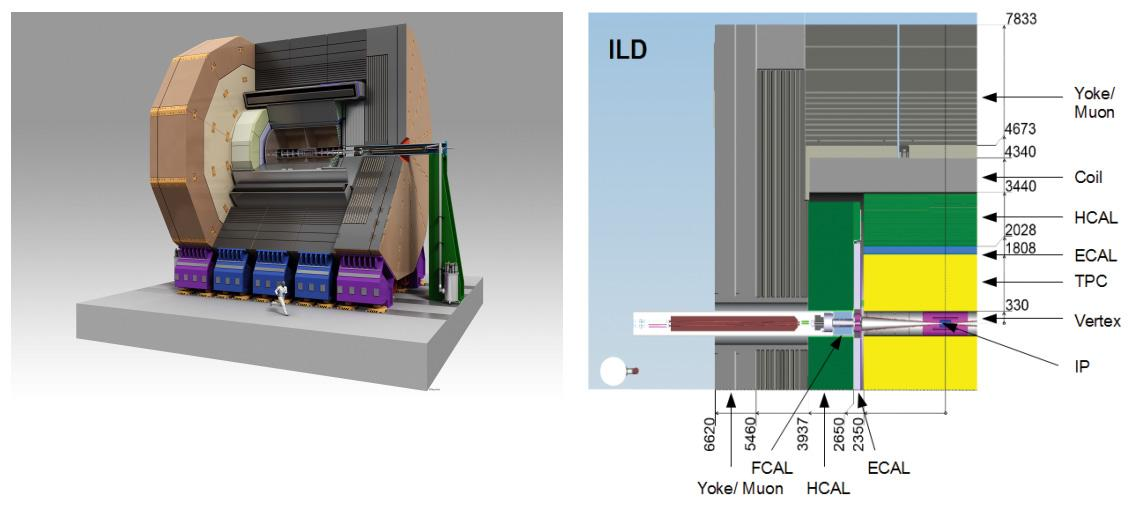
\includegraphics[width=0.95\textwidth,keepaspectratio]{Experiments/fig/ILD}
  \caption[ILD Detector]{The International Large Detector Concept (left). Schematic of the ILD showing the key components in a one-quarter view of a vertical section of the detector (right). Dimensions ar in mm \cite{Behnke:2013xla}}
  \label{Fig:ILD}
\end{figure}

The ILD (shown in \reffig{Fig:ILD}) is a general purpose detector which is cylindrical in design with radius 8m and length 14m. The different sub-detectors are arranged in a concentric manner in the main barrel of the detector, and are positioned with the vertexing technology closest to the beamline, followed by trackers, then electromagnetic and hadronic calorimeters, then the magnetic field coils which supply a 3.5T B-field and finally muon tail catchers. The detector has two endcaps with a similar layer structure at each end of the barrel creating a hermetic seal.

In order to provide precision measurements of the various processes proposed in the \ac{ILC} and \ac{CLIC} physics schemes, there are several strict requirements imposed upon the performance of the detector:

\begin{itemize}

\item \textbf{Momentum Resolution}: $\sigma_{p_t}^2/ p_{t}^2 \sim 2 \times 10^{-5} GeV^{-1}$, key for precision Higgs recoil mass measurements

\item \textbf{Jet Energy Resolution}: $\sigma_E/E \sim 3-4\%$, allows separation of hadronic W/Z decays

\item \textbf{Impact Parameter Resolution}: $\sigma_{b} < 5 \oplus \frac{10}{p\sin\theta^{\frac{3}{2}}}\mu m$, allows accurate flavour tagging for short lived particles

\item \textbf{Hermetic Coverage}: Needed for processes with a strong angular dependence or missing energy component 

\end{itemize}

Detailed specifications for the detector can be found in the \ac{ILD} Letter of Intent \cite{ILD}. Here we will give a brief overview of the key components, their functions, and the methods used for making the most of the information they provide.

\subsubsection{Vertexing}

The vertexing technology is used to gain information about heavier particles such as b-quarks which have very short lifetimes ($\sim$10$^{-12}$s) and so decay close to the beamline before they can reach the trackers or calorimeters. As such, the vertexers are placed extremely close to the beamline and work by looking for displaced vertices from the initial \ac{IP} which correspond to the point at which the heavy flavour paricles decayed. Due to their proximity to the beam line it is always necessary for the vertex detectors to be radiation hard as they are exposed to stray high energy particles from the beam. The vertexers also act as trackers for short lived particles that fail to reach the main trackers and so are required to be highly granular to separate particles that have had very little time to spread out since the \ac{IP}. The design for the vertex detectors is yet to be finalised as there are numerous competing technologies under consideration, but the target performance is to achieve a track impact parameter resolution of

\begin{equation}
\sigma_{b} < 5 \oplus \frac{10}{p\sin\theta^{\frac{3}{2}}}\mu m
\end{equation}

where $p$ is the track momentum in GeV, $\theta$ is the angle between the track and the vertex detector plane and the first and second terms describe contributions from the transverse impact parameter resolution and multiple scattering effects respectively.  In practice it is found that to achieve this impact parameter resolution a spatial resolution of at least 3 $\mu m$ is required. As well as achieving a sufficienct impact parameter resolution, the vertexing detectors are also required to have sufficient granularity and low enough occupancy rates to allow separation of individual tracks passing through the detector. On top of these requirements for the vertexing and tracking performance, the design for the vertexer must also avoid any negative impact on later parts of the detector. In particlular, the material budget of the whole detector system is limited to be less than one radiation length to avoid unwanted production of electromagnetic showers prior to the \ac{ECAL}. The detector layout used for the baseline studies in the \ac{ILD} \ac{TDR} assumes six layers of 50$\mu m$ thin silicon pixels arranged in pairs. The layout and details of the structure are shown in more detail in \reffig{fig:VTX} and \reftab{tab:aVTX}.

\begin{figure}
  \centering
  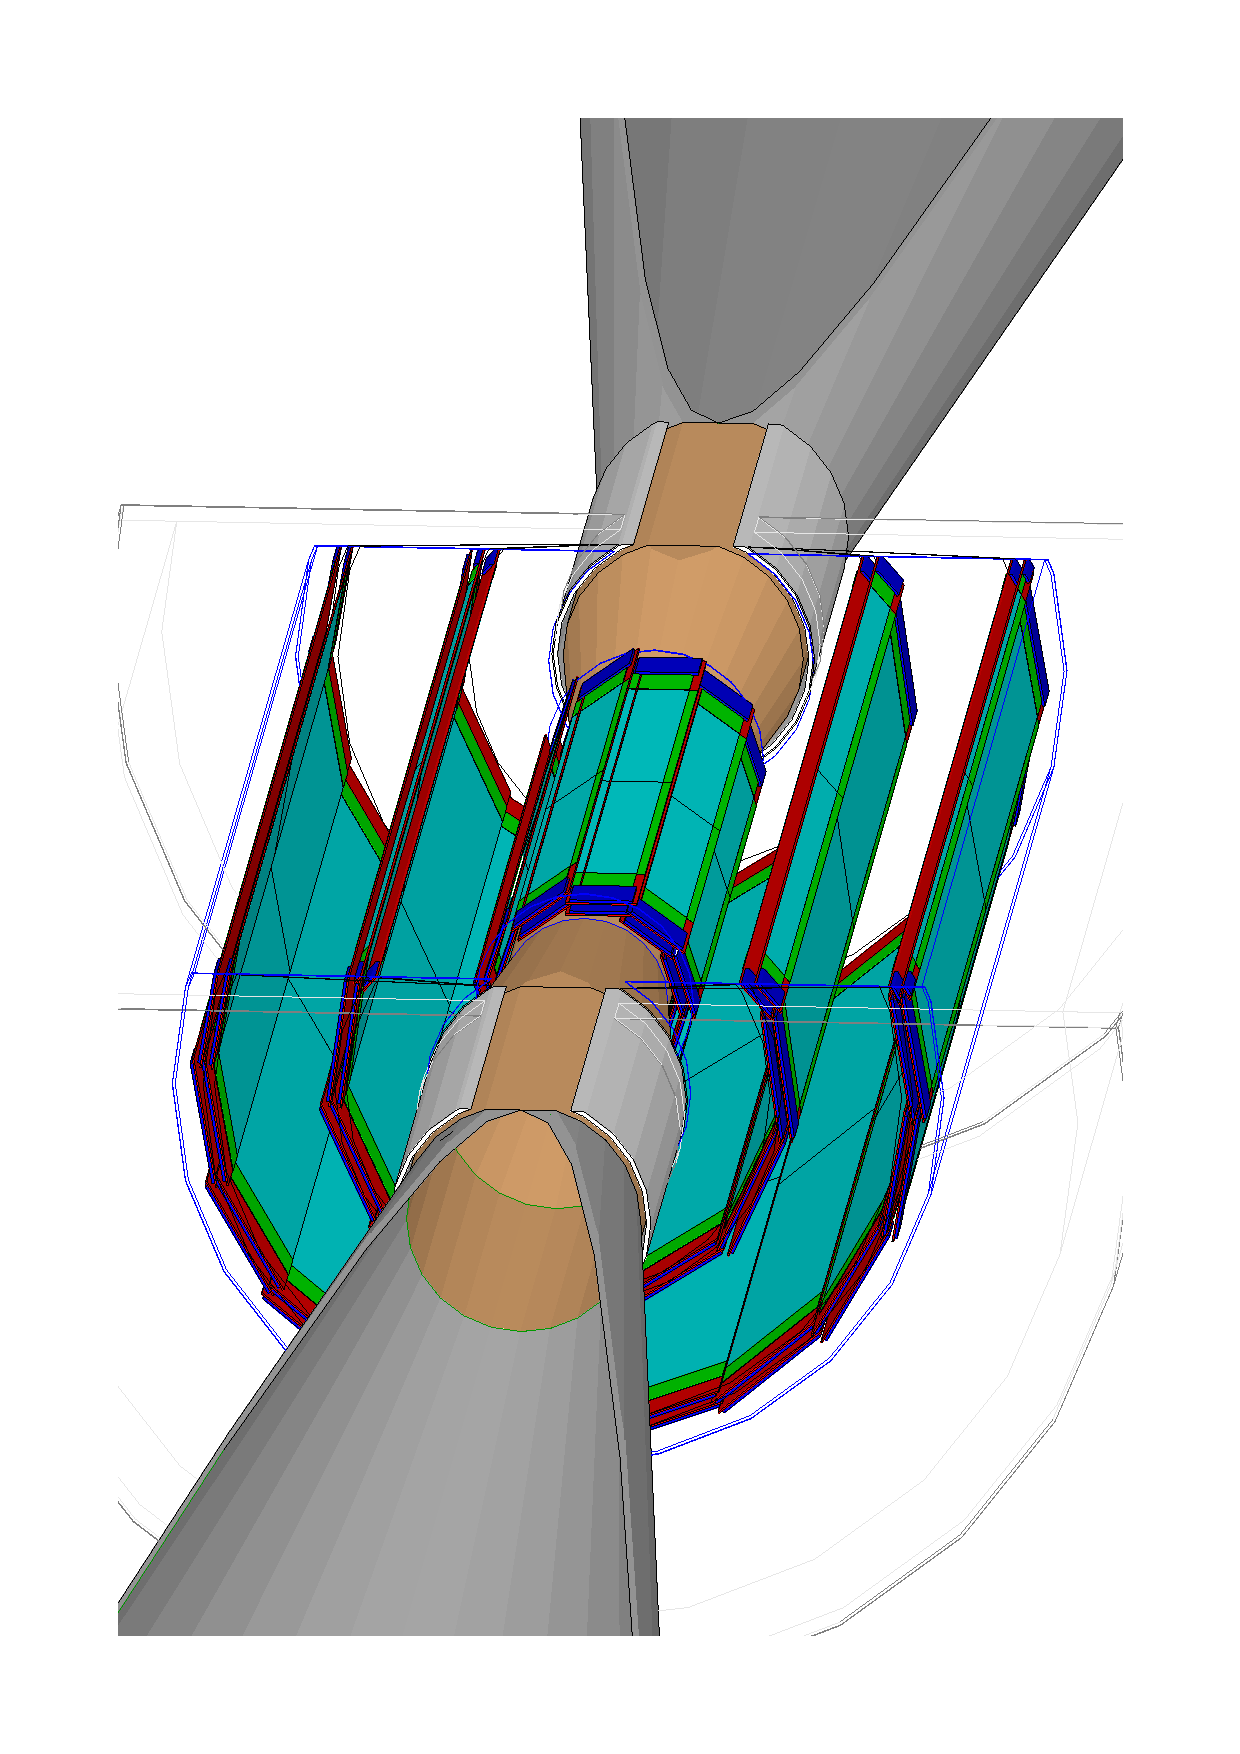
\includegraphics[width=0.3\textwidth,keepaspectratio]{Experiments/fig/Vertex}
  \caption[ILD Vertex Detector]{Proposed vertex detector geometry for ILD \cite{ILD}}
  \label{fig:VTX}
\end{figure}

\begin{table}
  \caption{Properties of the CLIC vertex detector assuming three pairs of layers \cite{ILD}}
  \centering

  \begin{tabular}{l l l l l l l}
    \toprule
    layer           & radius [mm]         & ladder length [mm]  & read-out time [$\mu s$]  \\
    \midrule
    1 & 16.0 & 125.0 & 25-50 \\
    2 & 18.0 & 125.0 & 25-50 \\
    3 & 37.0 & 250.0 & 100-200 \\
    4 & 39.0 & 250.0 & 100-200 \\
    5 & 58.0 & 250.0 & 100-200 \\
    6 & 60.0 & 250.0 & 100-200 \\
    \bottomrule
  \end{tabular}
  \label{tab:aVTX}

\end{table}


\subsubsection{Tracking}

Tracking in \ac{ILD} is performed by multiple subsystems. We have already discussed the vertexing systems which act as trackers for low transverse momentum and short lived particles, however the majority of the tracking is performed by a large \ac{TPC}.  This is a large gas filled cylinder extending from r=395 mm to r=1739mm with an electric field applied across it and readout electronics at each end of the cylinder on the endcaps. As particles pass through the gas, they ionize it producing charged particles. The electric field then causes these particles to drift to each end of the detector where they are collected by the electronics. By measuring the position and time at which the charged particles arrive, the track of the original ionizing particle can be reconstructed. A magnetic field is also generated across the chamber to deflect the charged particles so that the momentum and charge of the particle can be estimated. The magnetic field used in the ILD is a 3.5T coil placed outside the calorimeters to minimize the material budget in front of the calorimeters. The use of a \ac{TPC} provides several benefits over alternative technologies such as silicon tracking (the technology used in the \ac{SiD} tracker.) Because the ionization occurs across the whole track, it is possible to reconstruct the particles path from numerous spacial points to provide a precise meaurement of the path taken. This is not the case for a silicon tracker where the number of data points is proportional to the number of tracking layers present, however this is compensated for by the fact silicon trackers typically have a higher spatial resolution on each point ($\sim 1~\mu m$) compared to TPCs ($\sim 1~mm$.) TPCs also benefit from having a low material budget compared to silicon trackers. In \ac{ILD} the gas used will be Ar:CH$_{4}$:CO$_{2}$ (95:3:2) which gives a material budget of $\sim 0.04(0.15)X_0$ radially(longitudinally.) The choice of readout technology is yet to be finalised with several options being pursued (Micro-Pattern Gas Detectors, MicroMegas\cite{Giomataris:1995fq} and GEM\cite{Sauli:1997qp}) however in all cases it is expected that there will be 10${^{-6}}$ channels of diminsion $\sim$1$\times$6 mm$^{2}$. This system will allow a single point resolution of $<$100$~\mum$(0.5 mm) and two hit resolution of 2 mm (6 mm)  in the x-y (r-z) planes, and a resolution of 5$\%$ on dE/dx.

The \ac{TPC} is supplemented by a series of silicon based tracking systems whcih act to provide high spatial resolution points at the entrance and exit of the TPC which yields an improved momentum resolution and an improved performance from the \ac{PFA}s, provide time stamping for bunch tagging and assist in calibration of the \ac{TPC}. These additional subdetector systems come in four parts. In the barrel region, between the vertexer and the \ac{TPC} lies the \ac{SIT} which provides two high spatial resolution points at r= 165 mm and r=309 mm, while between the \ac{TPC} and the \ac{ECAL} lies the \ac{SET} which provides a single spatial point at r=1844 mm. Both of these systems are based on double sided silicon microstrips and provide a resolution of $\sim$ 50 um. The \ac{FTD}covers the very forward region of the detector down to 0.15 radians and consists of 7 disks positioned in the innermost tracking region, the first three using silicon pixels and the end 4 using silicon microstrips. The \ac{ETD} is similar in structure to the \ac{SET} but is positioned outside the \ac{TPC} endcaps rather than the barrel to provide high spatial resolution for particles exiting the tracker into the endcap calorimeters. The positioning of all these subdetector systems can be seen in \reffig{fig:silicontracking}.

\begin{figure}
  \centering
  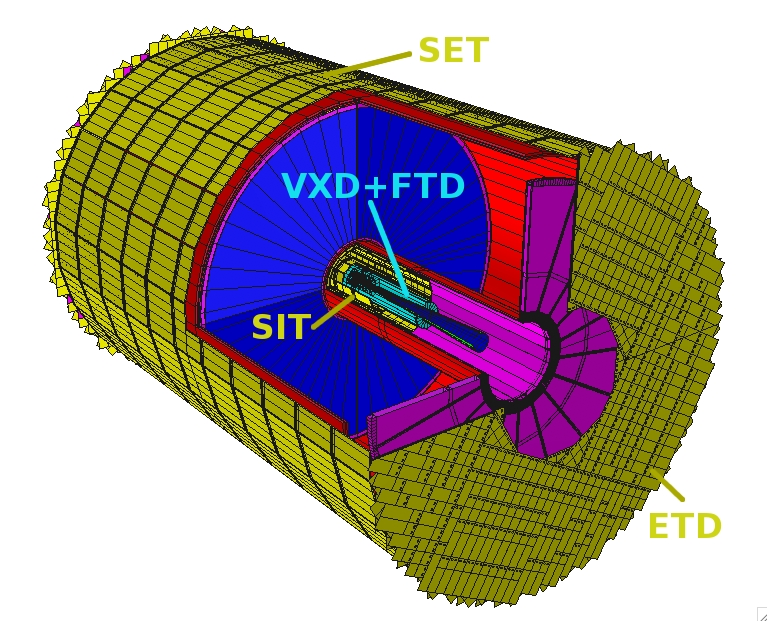
\includegraphics[width=0.5\textwidth,keepaspectratio]{Experiments/fig/SiliconTrackers}
  \caption[Silicon Tracking Systems For ILD]{Silicon Tracking Systems For ILD \cite{ILD}}
  \label{fig:silicontracking}
\end{figure}

The combined performance of the vertexer, \ac{TPC} and silicon tracking systems gives a momentum resolution of $\sigma_{p_t}^2/ p_{t}^2 < 2 \times 10^{-5} GeV^{-1}$ and a tracking coverage reaching to as low as $\cos\theta<$0.996.


\subsubsection{Calorimetry}
\label{det:ecal}
The function of calorimeters is to measure the energy of particles by passing them through a medium in which they will deposit some of their energy. As the way that particles interact with other matter is determined by the type of particle invloved, the calorimeters are usually split into two two sections, the \ac{ECAL} and \ac{HCAL}, that are designed to interact with electromagnetic particles (electron, photons) and hadrons respectively. As we will later be presenting work on a proposed novel design for a \ac{DECAL} it is pertinent to discuss in greater detail the relevant processes and terminology involved in electromagentic calorimetry to understand what issues there are with current \ac{ECAL} technologies and how the \ac{DECAL} might improve upon them.

When an electron interacts with matter it will typically radiate a photon via \ac{BS}. This photon then can then decay into an electron-positron pair which will in turn radiate further photons. This cascade process results in the formation of what is refered to as an electromagnetic shower. The shower will continue to develop until the energy of the shower particles reaches a critical value, E$_{C}$, at which the energy losses of the particle begin to be dominate by ionization rather than beamsstrahlung. The development of the electromagnetic shower can be characterised using several parameters. The most commonly used of these is the the radiation length, $\chi_0$, which is defined as the distance an electron can travel through a material before it's energy has reduced by a factor of 1/e via beamsstrahlung (or equivalently to 7/9 the mean free path for pair production of a photon.) The interaction length can be expressed as a function of a materials nuclear parameters \cite{Groom:1998it}:

\begin{equation}
  \chi_0= \frac{kA}{Z(Z+1)\ln{287/sqrt{Z}}}
\end{equation}

Where k is a constant equal to 716 gcm$^{-2}$, A is atomic mass, and Z is atomic number.

For the purposes of designing a detector, perhaps the most relevant parameters are those related to the size of the showers as these determine the dimensions required for the calorimeter to contain the shower. The longitudinal detector requirements are decided by the rate of energy loss for a particle which is given by the Bethe-Bloch equation which can be simplified to\cite{Beringer:1900zz}:

\begin{equation}
  \label{bethebloch}
\frac{dE}{dx}=E_0 b \frac{(bx)^{a-1}e^(-bx)}{\Gamma(a)}
\end{equation}

Where x is the material depth in units of $\chi_0$, $E_0$ is the initial energy of the particle, and a and b are properties of the absorbing material. The exponential term means that it is typically not possible to capture 100\% of the energy in a shower, instead an acceptable level of loss must be decided and the detector designed accordingly. For example, a typical energy scale for \ac{CLIC} would be $\sim$ 100 GeV. For a working point of 5\% loss a calorimeter depth of $\sim$17 $\chi_0$ is required, while for an improved performance of just 1\% loss a depth of $\sim$20 $\chi_0$. The transverse profile of the shower is described by the Moliere radius, the radius in which 90\% of a particles energy will be deposited:

\begin{equation}
R_M=\frac{21MeV}{E_c}\chi_0
\end{equation}

In general, it is necessary to have a Moliere radius that is smaller than the typical separation of particles produced in a collision so as to avoid overlapping of showers. For \ac{ILD} this is espeically true where Pandora \ac{PFA} relies on accurate association of tracks to calorimeter deposits which is only possible if the deposits from nearby particles can be distinguished.

For \ac{ILD} the \ac{ECAL} and \ac{HCAL} are both sampling calorimeters. This means that the structure is divided into layers of two alternating materials known as the absorber and active material. The absorber is typically a thick piece of high Z material that acts to initiate an \ac{EM} shower. The active material is then a thin low Z material that is easily ionizable and so acts to collect charge deposited from the shower. The active layer will then be instrumented to collect and readout the charge deposited within it. In order to reconstruct the energy of the initial particle that produced the shower, one would ideally just sum the deposits from each of the active layers, however in reality there will also be some energy deposited within the absorbing material that must be accounted for. This is done by scaling the energy deposited by the expected ratio of the energy deposited in the active layer to the total energy deposited in the active and absorbing layers combined. The scale factors will usually be determined as part of a calibration procedure for the detector in which muons are passed through each layer. The application of these scale factors introduces an uncertainty in the reconstructed energy as they represent an average scale correction, whereas the actual ratio of the energy deposited in the active and absorbing layers will be determined by additional factors that can't be easily measured. One example would be the path taken by the particle which can change the relative distance travelled by the particle in the active and absorbing layers.

The overall performance of a calorimeter is given by the energy resolution. This represents the quadrature sum of all sources of uncertainty in the energy reconstruction which are usually borken down by their energy dependence and expressed as follows:

\begin{equation}
  \frac{\sigma_E}{E}=\frac{a}{\sqrt{E}} \oplus \frac{b}{E} \oplus c
\end{equation}

Where a, b and c are typically referred to as the stochastic, noise and leakage terms. The energy dependence of the background and leakage terms are straightforward to understand. Noise typically arrises from the electronics used for collecting and reading out the hits in the active layers. This means that it is independent of the energy of the incident particles energy and so the absolute uncertainty doesn't vary with E. The leakage term accounts for the amount of energy lost from the calorimter not being deep enough to contain the shower. One can see from \refeq{bethebloch} that the energy lost will scale with the incident particles energy.

The stochastic term is slightly more complicated as it represents a combination of effects. The first of these is the intrinsic resolution of the detector which is determined by the physics of how an \ac{EM} shower develops. The number of particles produced in a shower (N)  is proportional to the energy of the incident particle (E), however the formation of bremstrahlung photons and electron-positron pairs is a quantum mechanical process and so is inherently statistical. As a result N will follow a Poisson distribution and so the uncertainty on it will be 1/$\sqrt{N}$. As N is proportional to E, this means there is an inherent uncertainty in the energy proportional to 1/$\sqrt{E}$. There are also further statistical contributions that arrise from using a sampling approach. For low energy particles produced in the absorber there is a chance that they be absorbed before making it to the active layer and so will not be accounted for in the scale factors. The uncertainty associated with this can be described by $\sqrt{E_{c}x/E}$. This factor is further added to by the effect mentioned above where x will vary from particle to particle depending on the path it takes through the detector. Because the energy deposited in a material as a function of the material depth is described by a landau distribution, uncertainties from varying path lengths are often referred to as landau fluctuations with the form $\sigma_{landau}/\sqrt{E}$.

\subsubsection{ECAL}
The \ac{ILD} \ac{ECAL} is a highly granular calorimeter poitioned at r=1847mm which consists of 30 active layers separated by layers of absorbing material. Tungsten is chosen for the absorber due to it's short radiation length, $\chi_0$=0.35cm. The first 20 absorber layers are 0.6$\chi_0$(2.1mm) thick while the later layers are  1.2$\chi_0$ to contain higher energy \ac{EM} showers while maintaining a compact design. The structure of the \ac{ECAL} is shown in \reffig{Fig:ECAL}. The active material will conisist of 5x5 mm$^2$ pitch silicon pixels and yields a resolution of

\begin{equation}
  \frac{\sigma_E}{E}=\frac{16.6\pm 0.1}{\sqrt{(E(GeV)}}\oplus(1.1\pm 0.1)\%
\end{equation}

While this is currently the default used in simulations for physics analyses, the choice of active material is yet to be finalised. A variation that uses 10x45 mm$^2$ silicon scintillator strips which would be rotated by 90${^o}$ in each successive layer to produce an effective cell size of 10x10 mm$^2$ with photomultipliers attached to each strip for readout also exists. The energy resolution for this form of the detector has been measured to be

\begin{equation}
  \frac{\sigma_E}{E}=\frac{14}{\sqrt{E}}\oplus2\%
\end{equation}

however the pixel version is typically favoured due to it's simpler design which doesn't require additional processing to produce the desired granularity.

\begin{figure}[h]
  \centering
  \begin{tabular}[c]{cc}
  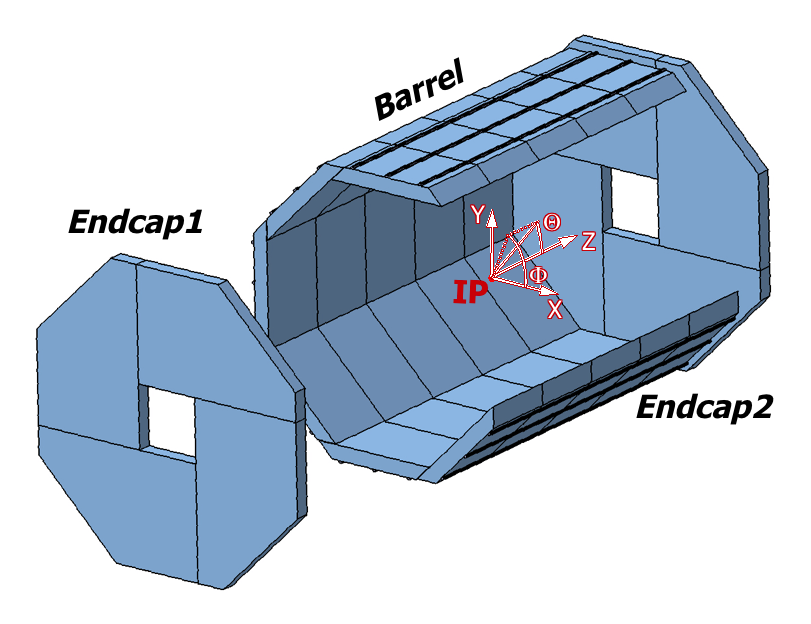
\includegraphics[height=5.5cm]{Experiments/fig/ECALview_global_annot} &
  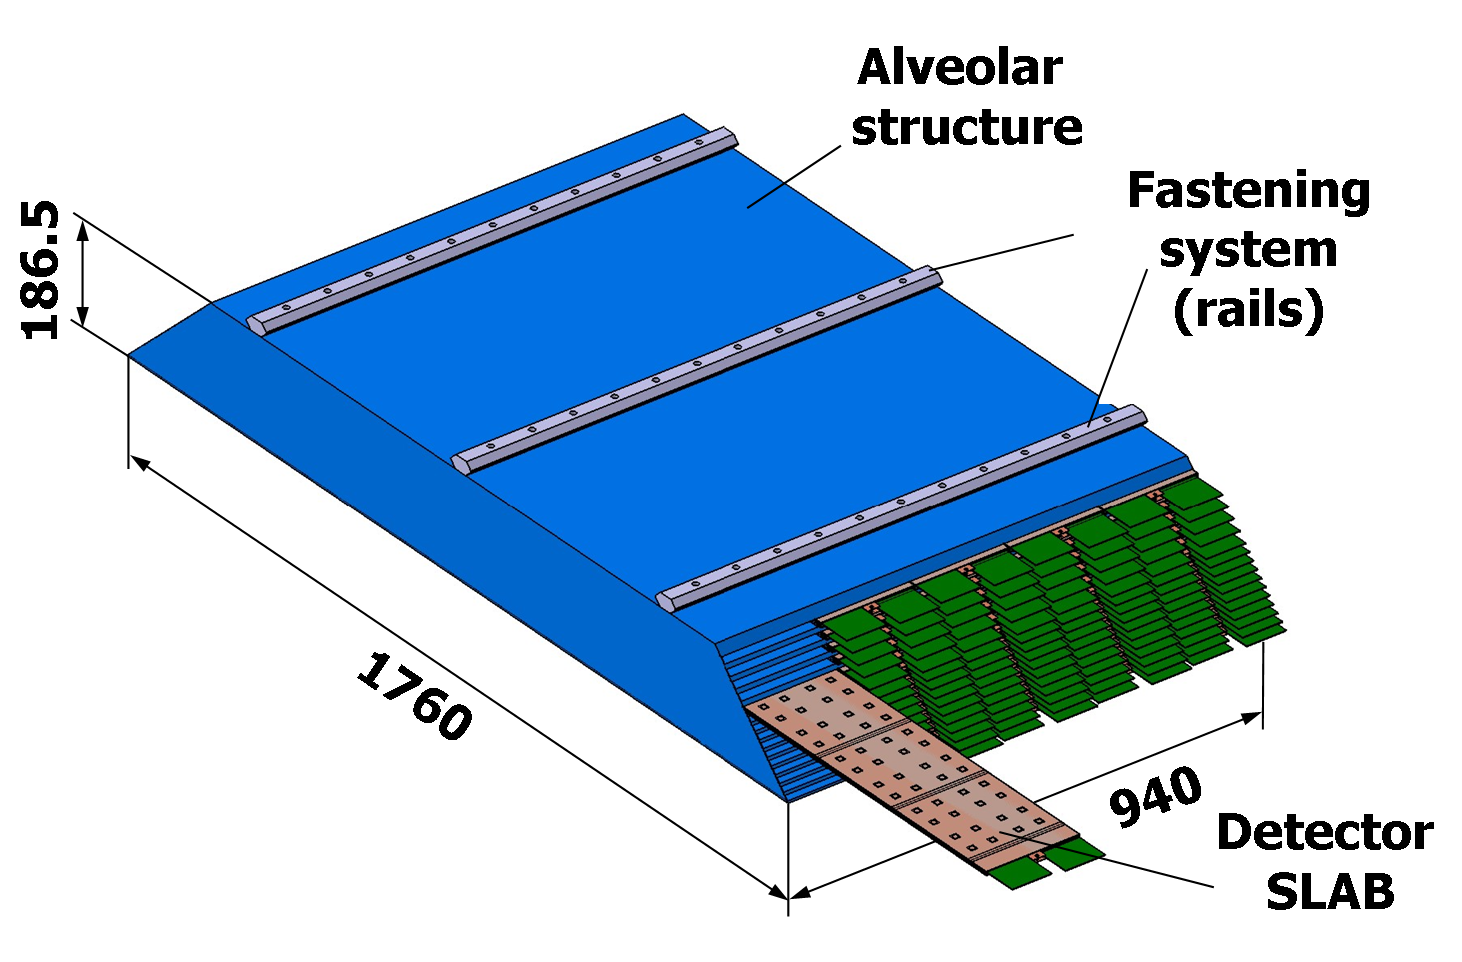
\includegraphics[height=5.5cm]{Experiments/fig/ECALview_module_annot} 
  \end{tabular}
  \caption[ECAL Structure]{The Overall ILD Structure (left) and one individual module (right).The ECAL is made up 40 modules, each containing 30 detector slabs. The modules are combined into groups of 5 referred to as a stave which extend along the full length of the barrel. There are then 8 of these staves arranged in a circle to create the circumference of the barrel \cite{ILD}.}
  \label{Fig:ECAL}
\end{figure}

Later on (see \refsec{sect:DECAL}) we will discuss our work on developing an alternative form of the silicon pixel technology with ultra high granularity 50x50~$\mu^2$m pixels which acts as a digital machine and purely counts the number of particles absorbed in the active medium from the showering in the absorber and deduces the energy of the original particle from this.  This form of the technology has already begun to be studied \cite{2011JInst...6.5009B}. It is expected to be cheaper than the standard silicon pixel tehnology as it is based on \ac{CMOS} technology which is already mass produced commercially, and has the potential for improved performance over it's analogue counterpart due to reduced sensitivity to landau fluctuations.

\subsubsection{HCAL}

\begin{figure}[h]
  \centering
  \begin{tabular}[c]{cc}
    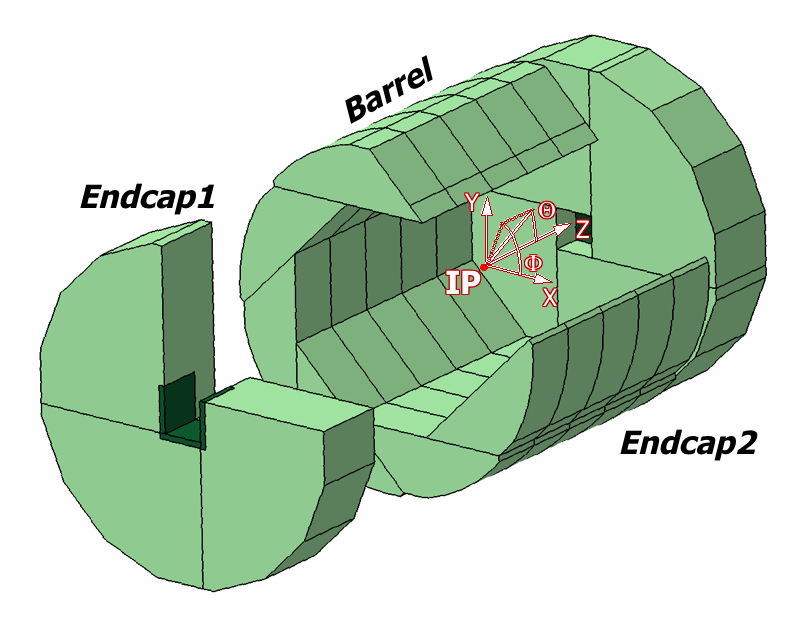
\includegraphics[height=5.5cm]{Experiments/fig/DHCALview_global.png} &
    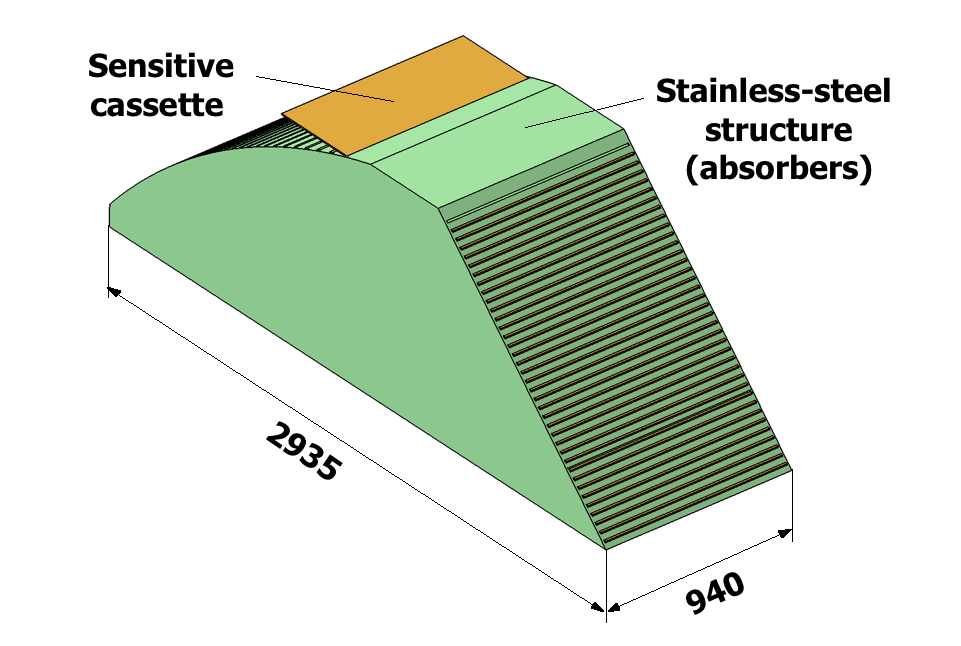
\includegraphics[height=5.5cm]{Experiments/fig/DHCALview_module.png}
  \end{tabular}
  \caption[HCAL Structure]{The Overall ILD HCAL Structure (left) and one individual module (right).The HCAL is made up 40 modules, each containing 30 detector slabs. The modules are combined into groups of 5 referred to as a stave which extend along the full length of the barrel. There are then 8 of these staves arranged in a circle to create the circumference of the barrel \cite{ILD}.}
  \label{fig:HCAL}
\end{figure}

The \ac{HCAL} is immediately outside the ECAL at r=2058 mm and has a similar overall modular structure to the \ac{ECAL} as shown in \reffig{fig:HCAL}. Each module consists of 48 stainless steel absorber plates of thickness 20 mm interspaced with 3 mm silicon scintillators with a transverse segmentation of 30x30 mm$^2$. This gives the \ac{HCAL} a total depth of $\sim$5 $\lambda_I$ (where $\lambda_I$ is the nuclear interaction length, the equivalent of $\chi_0$ for hadronic showers, which is typically much longer than $\chi_0$) and an energy resolution of 49\%/$\sqrt{E}$.

\subsubsection{Muon Detection}
Muon detection is perhaps the easiest process to perform at the ILC. Because the event environment at the ILC is typically clean with few high energy particles, few particles other than muons are capable of penetrating through the inner detector layers and the coil generating the magnetic field. As a result the muon detetors are produced by instrumenting the return yolk (r=4424 mm) that already surrounds the detector to contain the magnetic field. The number of muons produced in an event is also relatively small which means that the cell size for the muon detectors can be moderately large without the risk of multiple occupancy. The instrumentation is done by placing 10 layers of resistive plate chambers into the return yolk with strip sizes of the order 3-4 cm. This system is sufficient for accurately detecting muons and contributing to the measurement of their momentum. This system provides $\sim$100\% efficiency for identifying muons with momentum $>$3 GeV. Below this the muons do not have enough penetrating power to traverse through the yolk. This identification performance can extended down to 1.5 GeV when information from the calorimeters is included as well.

\subsubsection{Very Forward Region}

Further instrumentation is present in the very forward regions of the detector for beam monitoring and to provide additional angular coverage. There are two main detectors of interest in this region.

The first of these is the LumiCal. As the name suggests this is designed for measuring the beam luminosity. The LumiCal consists of 30 layers of tungsten interspaced with silicon sensors covering the angular range of 32 to 74 mrad. The luminosity is determined by measuring the rate of Bhabha scattering in this region then scaling by the predicted cross section for the Bhabha scattering for the same angular range. As the Bhabha scattering process is a first order electroweak interaction the theoretical uncertainty on this cross section is small allowing for a precise measurement of the luminosity. For the studies presented here which are performed at 1.4 TeV at CLIC, this method allows the luminosity to be measured to a precision of $\sim$0.3\%.

The second detector of interest is the LHCal. This is a supplementary component of the for the \ac{HCAL} which extends the coverage down to lower angles. The design for this is yet to be finalised, however it is expected to provide four radiation lengths of material covering the gap between the beam pipe and the \ac{HCAL} endcap will consist of 40 layers of 1 cm thick tungsten interspaced with silicon.

Along side these there are also several systems for performing beam monitoring- namely the BeamCal, GamCal and pair monitor, however as these are less relevant to the studies presented in this thesis we shall not discuss them in detail here. Details on all the forward components of \ac{ILD} can be found in the \ac{ILD} lettor of intent\cite{ILD}.


\subsection{CLIC ILD}

At \ac{CLIC} the detector designs were orginally based on the two \ac{ILC} detectors, \ac{ILD} and \ac{SiD}, but with a few changes to adapt for the different experimental conditions at \ac{CLIC}. In the case of \ac{ILD}, due to the large beam related backgrounds the vertex detectors were moved to be 15 mm further from the \ac{IP} to avoid pixel saturation. To account for the higher energy jets produced in interactions, the \ac{HCAL} depth was extended to 7.5 $\lambda_I$ to reduce leakage out of the back of the detector. To avoid increasing the radius of the magnetic solenoid (one of the main driving costs of the whole detector) the choice of absorber material in the \ac{HCAL} was switched to tungsten to provide the increased interaction length but over the same depth as in the orignal steel design. In the barrels, because the thickness does not affect the solenoid radius, the absorber was left as steel. To improve the charge identification of higher energy tracks, the magnetic field strength was changed to be 4T which was found to still be achievable using the original \ac{ILD} solenoid design. Further details on the CLIC version of \ac{ILD} can be found in the \ac{CLIC} \ac{CDR}\cite{CDR}.

This version of the \ac{ILD} detector is used for the analyses presented in Chapters \ref{Higgs Analysis} and \ref{chapter:topanalysis}. Since these analyses have been conducted, \ac{CLIC} has recently produced a new unified detector design that will be used for future studies. Overall the design is similar to that of \ac{ILD} but with a deeper \ac{ECAL} to allow for higher energy photon containment and the tracker has been changed from a \ac{TPC} to an all silicon tracker. As this version is not used in the studies presented here we will not give a detailed account of the detector but more information is avilable in \cite{Pitters:2018jxt}. Overall the impact of the change in dedector design is expected to be negligible for the studies presented here.






